\documentclass{article}

\usepackage{graphicx}
\usepackage{rotating}

\title{comparison of data sets}
\author{Alden Bradford}

\begin{document}
\maketitle

\abstract{
In a collaboration between Weiyi, Matt, and myself, we identified three publicly available datasets which include accelerometer data from controlled falls. Our hope is to be able to transfer information from these controlled studies to our problem domain, or at least see how these other datasets were successfully classified. Here I describe some insights these datasets provide about our problem.
}

\section{Factor analysis}
Now that we have some other datasets available, we can begin to explore them in the same way we have explored the Makusafe data. One of the things we tried was factor analysis on the features -- this allows us to see which features vary together. I scaled each feature to have mean zero and unit variance, then carried out factor analysis. Since the covariance matrix had ten eigenvalues greater than 1, I chose to look for ten factors. Here is a table comparing their factor loadings, scaled linearly so that each factor has a maximum loading of 1.

\begin{figure}[h!]
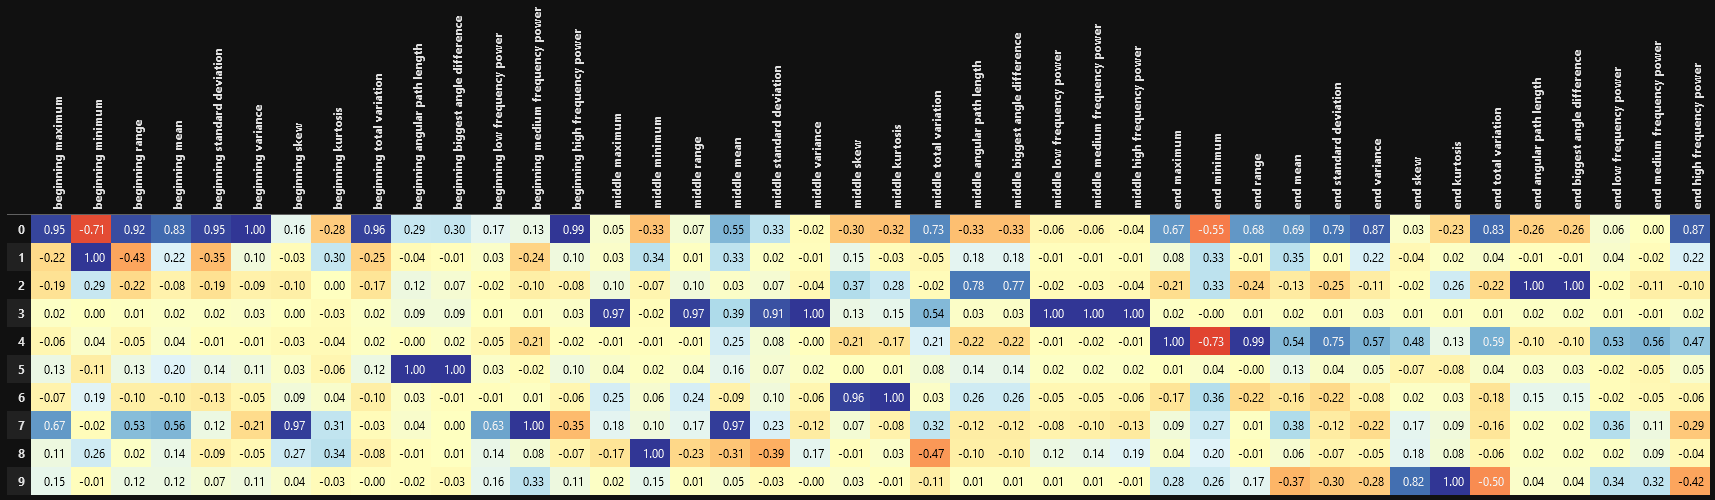
\includegraphics[width=\textwidth]{factors}
\end{figure}

We can see that several features are redundant, in terms of what they encode. Looking at row 6, for example, we see that the skew and variance are highly correlated for the middle section of the incident. This makes sense, because both should be dominated by the central peak of the acceleration curve.

For each factor, I chose the feature with the greatest loading to include in a plot. Then, I generated a scatterplot for each pairing. The result is in Figure \ref{pairplot}.

\begin{figure}
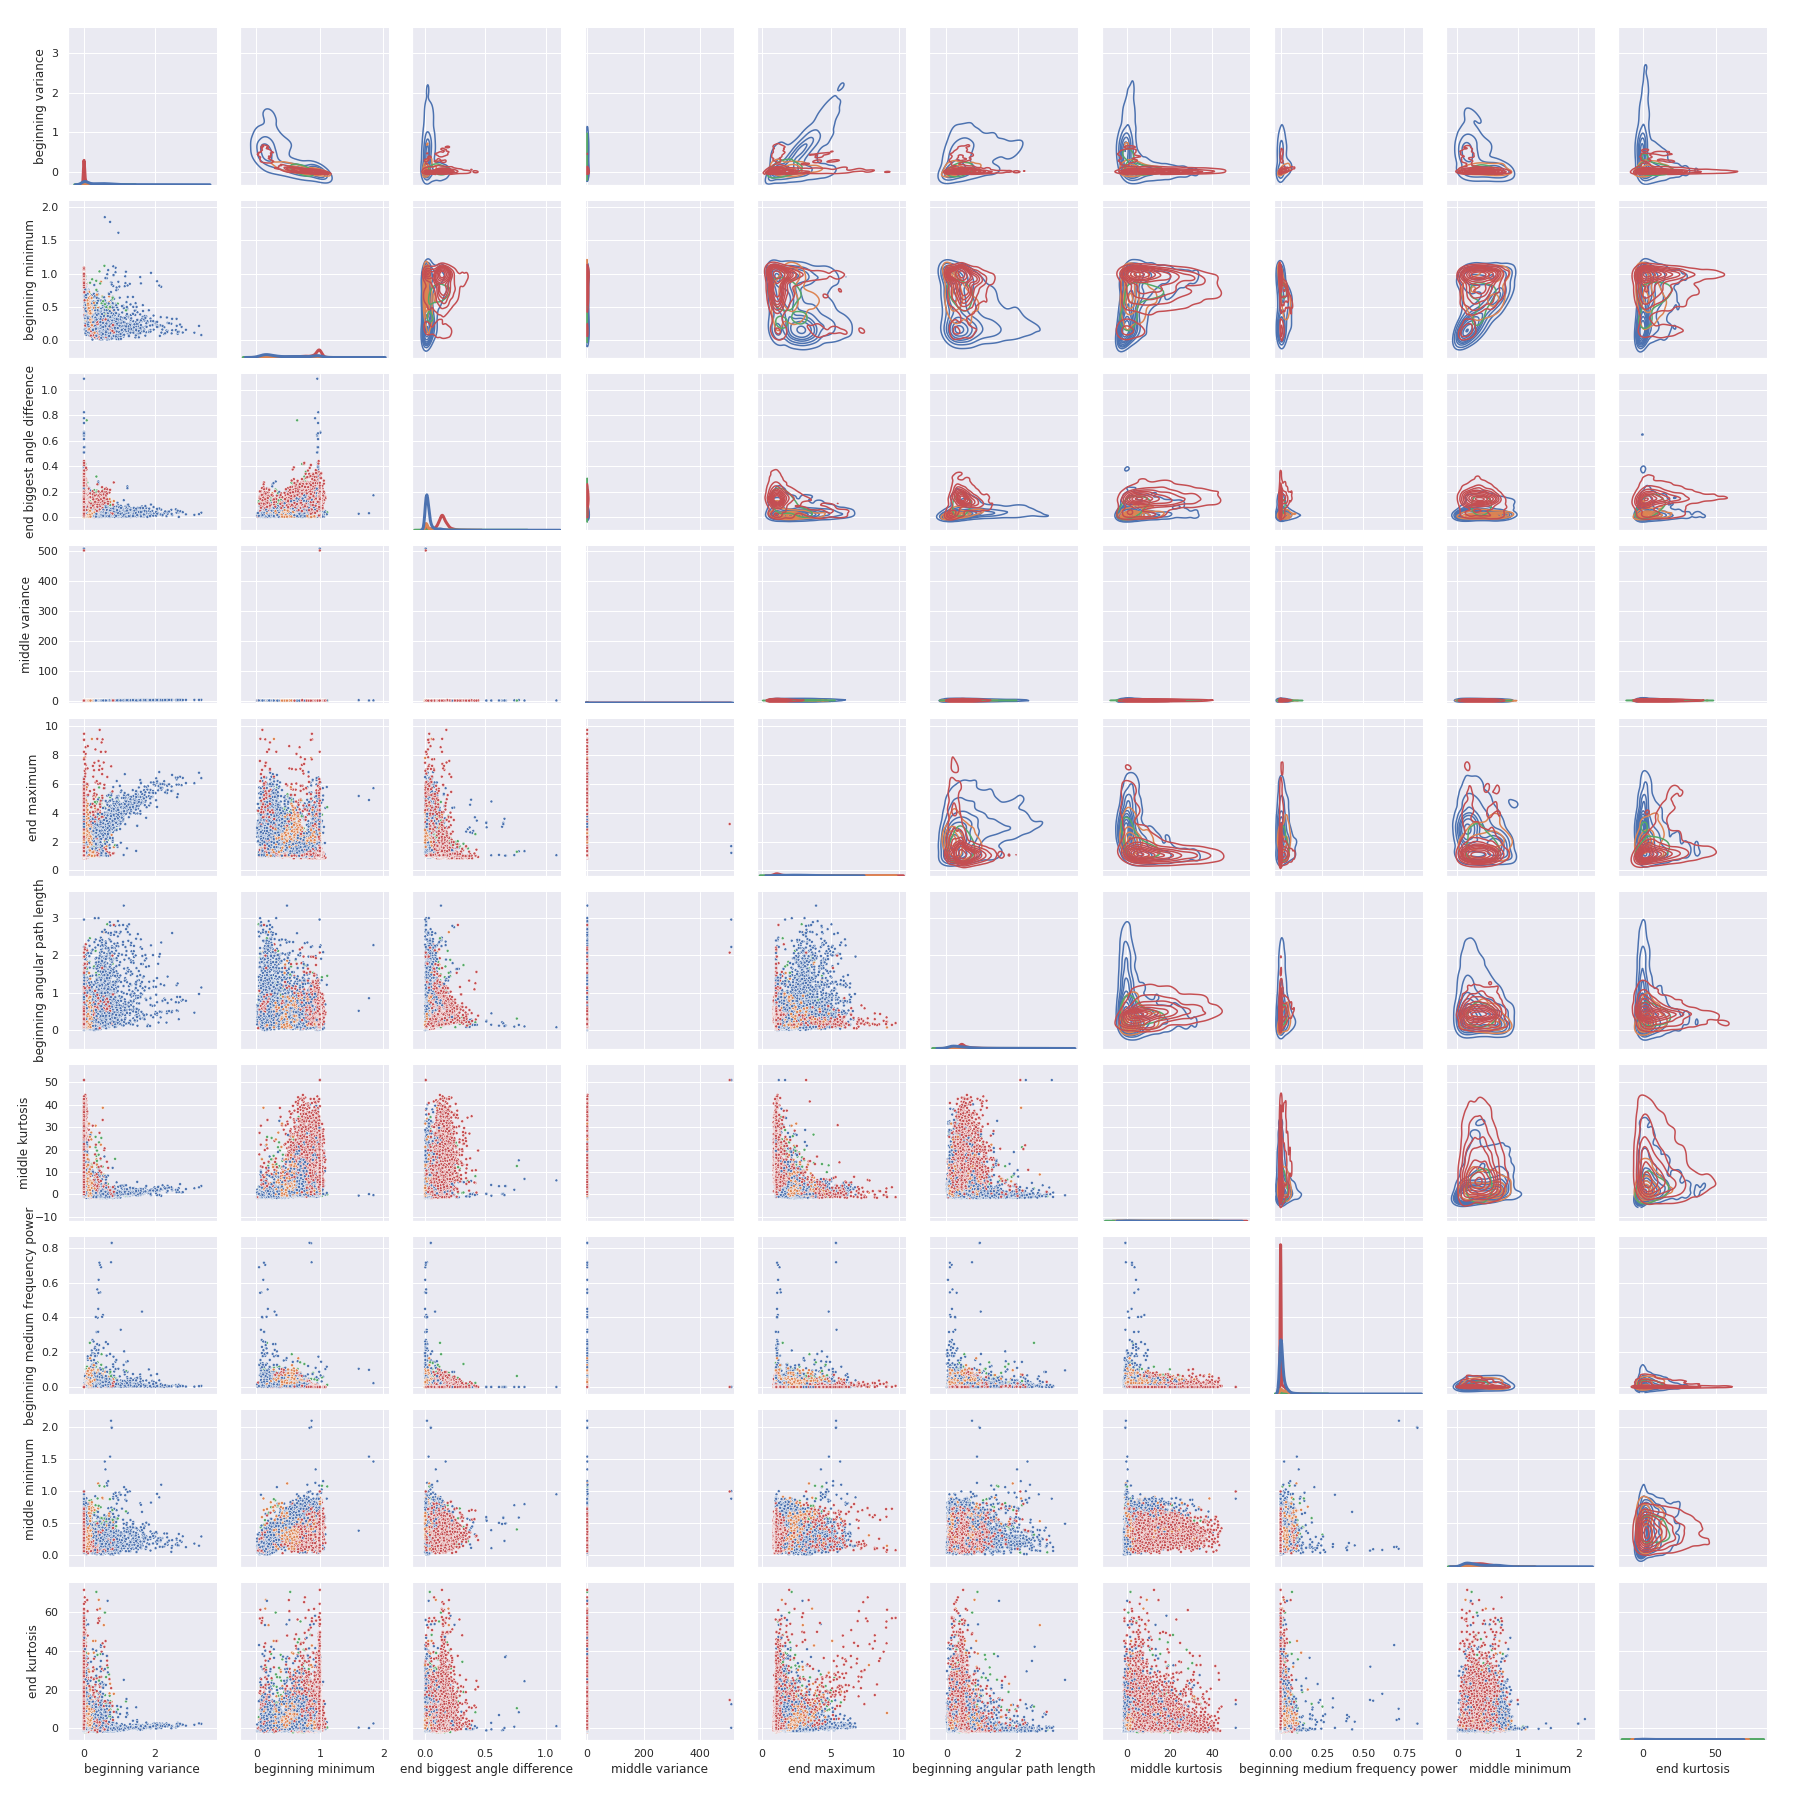
\includegraphics[width=\textwidth]{pair_plot_othersets}
\caption{A selection of features. Each point is an incident, each color its motion.}
\label{pairplot}
\end{figure}

For the rest of the document, we will focus on just one of these figures: the beginning variance versus the middle kurtosis. This one appears to show a good separation between the hazardous and non-harzardous incidents.

\section{Beginning variance, middle kurtosis}

It is important to remember that each chosen feature is just one representative of a class of related features. For example, the beginning variance aligns very well with several other features also computed on the ``beginning'' portion of the signal (the portion spanning from 4 seconds pre-incident to one second pre-incident). It aligns well with the total variation, as well as the range. We can consider this an indication of how much the acceleration was going up-and-down during whatever activity preceded the incident. Recall that this is strictly looking at the magnitude of the acceleration, so we do not expect it to be affected by rotation or positioning. It makes sense that this would be a negative predictor of hazards; if the person was moving vigorously, their base levels of acceleration would be higher and so they would necessarily have a higher chance of falsely triggering the acceleration threshold.

The kurtosis in the middle is highly correlated with the skew in the middle. The ``middle" here means the period extending from one second pre-incident to one second post-incident. A high skew or kurtosis would be caused by a small number of samples which are very different from the majority of samples. We can consider this an index for how high the peak acceleration was, compared to the usual fluctuations in acceleration during this interval.

\begin{figure}
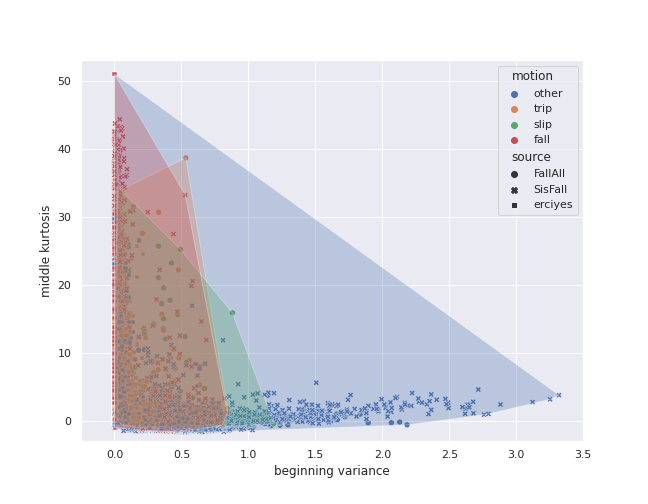
\includegraphics[width=\textwidth]{variance_vs_kurtosis_other_datasets}
\caption{The plot of begiinning-variance versus middle-kurtosis. Notice there are mostly blue dots in the lower-right, and mostly red dots in the upper-left.}
\label{othersets}
\end{figure}

See the results of this in Figure \ref{othersets}. It is clear that a high variance in the beginning interval is a predictor of a non-hazardous incident. In particular, there were no hazards with a beginning variance greater than 1. Compare this with the kurtosis during the middle interval, and we see that a kurtosis greater than about 15 is a very strong indicator that the incident was hazardous. This pattern shows up independently in each data set we considered; it is not an artifact of combining data from different sources. A similar plot showing only the points from each of our datasets on its own is included in Appendix \ref{other_set_plots}.

\section{The Makusafe data}

It is natural to ask: how does the makusafe data compare to this? Let's inspect a plot showing the same features, this time only looking at data from Makusafe. This is in Figure \ref{makusafe}. What we see looks familiar, in the sense that is is a similar shape -- it is just missing the major non-hazardous branch. We have mostly these high-kurtosis incidents, which in the other three datasets would almost certainly be classified as hazards. We have very few of the high-variance incidents which would be classified as false alarms. What we see instead is that the ``true hazards" are all mixed in with the false alarms. There would be no way, based on these two features, to distinguish them.

\begin{figure}
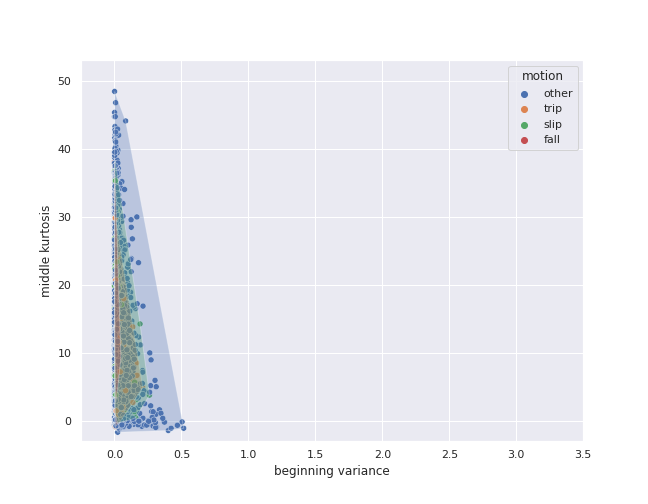
\includegraphics[width=\textwidth]{variance_vs_kurtosis_makusafe}
\caption{The data from Makusafe}
\label{makusafe}
\end{figure}

\section{Conclusions}

This was an exercise in data exploration. There are not many things we can conclude definitively. What follows are a few speculations based on this observation.

\subsection{The other data sets are fundamentally different -- what works for these may not work at all for the Makusafe data.}

The other studies we considered relied on computing simple statistics such as variance and skew. We can see from this simple demonstration that this makes sense for the data they have. When comparing these variables, a clear separation emerged.

We can see from this analysis that it would be unreasonable to suspect that same strategy to work for the Makusafe data. The data are simply not as well separated, at least not along the same features. This also suggests that, while support vector machines were appropriate for the other data sets, they may be inappropriate in our case.

\subsection{Potential causes}

Why do these sets behave so differently? I think it is safe to rule out differences due to position of sensor, or sampling frequency. The Erciyes data set, for example, had the same sampling frequency as the Makusafe data. Each of the other data sets had sensors mounted at a different point on the body -- the wrist, the waist, the chest. It would be very strange if the upper-arm was so very different.

I see three potential sources of the difference:
\subsubsection{controlled vs uncontrolled}
The other data sets used simulated falls, while the Makusafe data uses real observed falls. It could be that a simulated fall has very different characteristics from a real fall.

\subsubsection{wider range of non-hazardous activities}
The other data sets had a limited set of activities being performed -- walking, running, jumping, standing up, lying down, etc. The activites that a person does in a factory for example may not be well-represented by these so-called ``activities of dailiy living".

\subsubsection{unreliable classification}
It could be that many of the incidents in the Makusafe set which are classified as ``other" would be better classified as ``a fall, but not the kind of fall we are worried about.'' That is, it may be that a high kurtosis is in fact a good predictor of a fall, and the incidents in the Makusafe set were misclassified because of a misalignment about what we think should constitute an incident which is worth reporting.

\subsection{Future directions}
Based on this exploration, it would be unreasonable to think a suport vector machine, for example, could be trained on these other data sets and give a good model which predicts the ways that the Makusafe data are labeled. We should even reconsider many of our choices for features -- we chose them because they worked well for these other data sets, which we now have reason to believe will not lead to a good performance on our data. Alternatively, we should reconsider what our goal should be. Perhaps instead of trying to predict what the labels are, we should try to produce some easily-computed index of risk which could be used in aggregate to identify hazardous locations or activities, for example.


\appendix

\section{Separate plots of other datasets} \label{other_set_plots}

Since each of these data sets came from a different source, using different accelerometers under different testing cicumstances, it would be reasonable to suspect that the bahavior documented above -- the split of the data into two well-separated clumps -- could be due to only differences in the data collection methods. However, this does not seem to be the case. To one degree or another, we see this pattern in each data set independently. You can see this for yourself in Figures \ref{fallalld}-\ref{erciyes}.


\begin{figure}
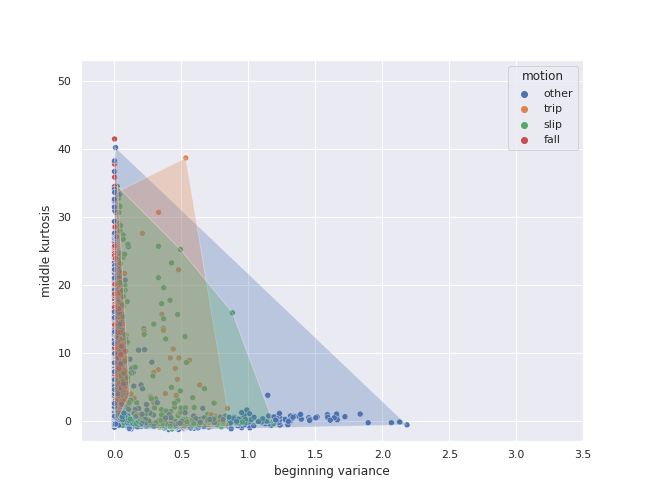
\includegraphics[width=\textwidth]{variance_vs_kurtosis_FallAll}
\caption{The data from FallAllD}
\label{fallalld}
\end{figure}
\begin{figure}
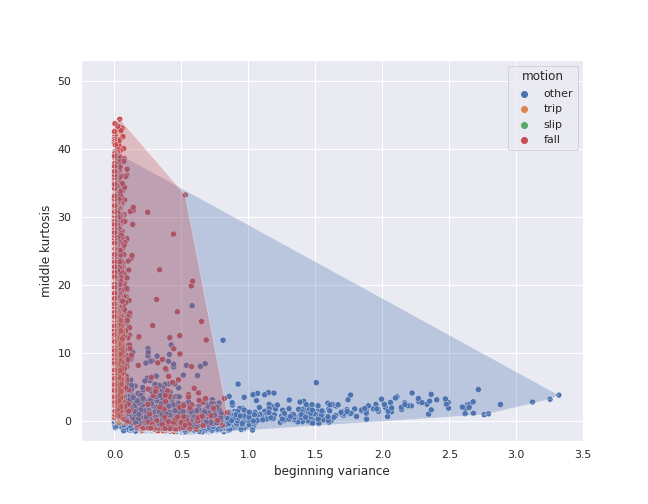
\includegraphics[width=\textwidth]{variance_vs_kurtosis_SisFall}
\caption{The data from SisFall}
\label{sisfall}
\end{figure}
\begin{figure}
\includegraphics[width=\textwidth]{variance_vs_kurtosis_Erciyes}
\caption{The data from Erciyes}
\label{erciyes}
\end{figure}

\end{document}